\section{Risk/Opportunity  management process \label{sect:strategy} }

\subsection{Roles and responsibilities  \label{sect:org} }

\subsubsection{LSST members}
The approach in DM is  that all LSST  members are free to identify risks through the DM risk management project in Jira.


\subsubsection{Risk Management Team}

The RMT is composed of the following: the DM Project Manager, the DM System Engineer and the DM Quality Assurance Manager{\color{red}Do we have such a role?}  . This list can be extended to some technical experts depending on the risk nature.

The RMT shall be led by the PC and be responsible for:
\begin{itemize}
\item Maintaining the DM risks in the LSST Register.
\item Any reissues of this document.
\item Issuing a DM Risk Report after each risk management meeting.
\item Completing a risk management cycle, as described in section \ref{sect:strategy}, at least once per development cycle.
\item Acknowledging new risks and monitoring registered risks, as specified in section \ref{sect:tasks}.
\item Recommends an assessment that the DMLT approves or modifies.
\end{itemize}
Risk management meetings are held by the risk management team (RMT) at least twice per year, and at least one month prior to regularly scheduled DMLT meetings. The risks actions may be  monitored monthly during the DMLT teleconference.

\subsubsection{DMLT}

It is the DMLT{\color{red} OR TCT ?} that has the authority to:
\begin{itemize}
\item Assess the acknowledged risk or, if any, approve the RMT risk assessment.
\item Decide on actions to mitigate risks as needed, approving proposed action from the RMT or formulating new actions.
\end{itemize}

\subsubsection{Local Risk Manager}
Each DM group shall designate a Local  Risk Manager (which could be the TCAM but need not be). This person shall be responsible for:

\begin{itemize}
\item Identifying and submitting in JIRA any new risks that will be reviewed by the RMT.
\item Validating the recommendations of the RMT on existing risks affecting the group.
\item Communicating to the RMT any action carried out to reduce identified risks, as well as their effectiveness.
\item When appropriate, or on request of the RMT, indicate for risk, a technical expert in the group that the RMT may contact directly for necessary clarifications.
\end{itemize}

In short, the Local Risk Manager is the contact point for the RMT, and guarantees that there is at least one person in the group management structure to communicate and track the CU risks.

\subsection{Risk management tasks \label{sect:tasks} }

To assure that mitigating actions are completed on a timely basis, risk management will take place on a cyclic basis.

Figure below defines the tasks and responsible that take place over a risk management cycle.
These tasks are based on the ECSS standards (ECSS-M-ST-80C) tailored to the DPAC and proposed here for LSST DM.
Risk management meetings will be held on a regular basis to address these tasks, thus there is one risk management meeting per risk management cycle.

\begin{figure}[H]
\begin{center}
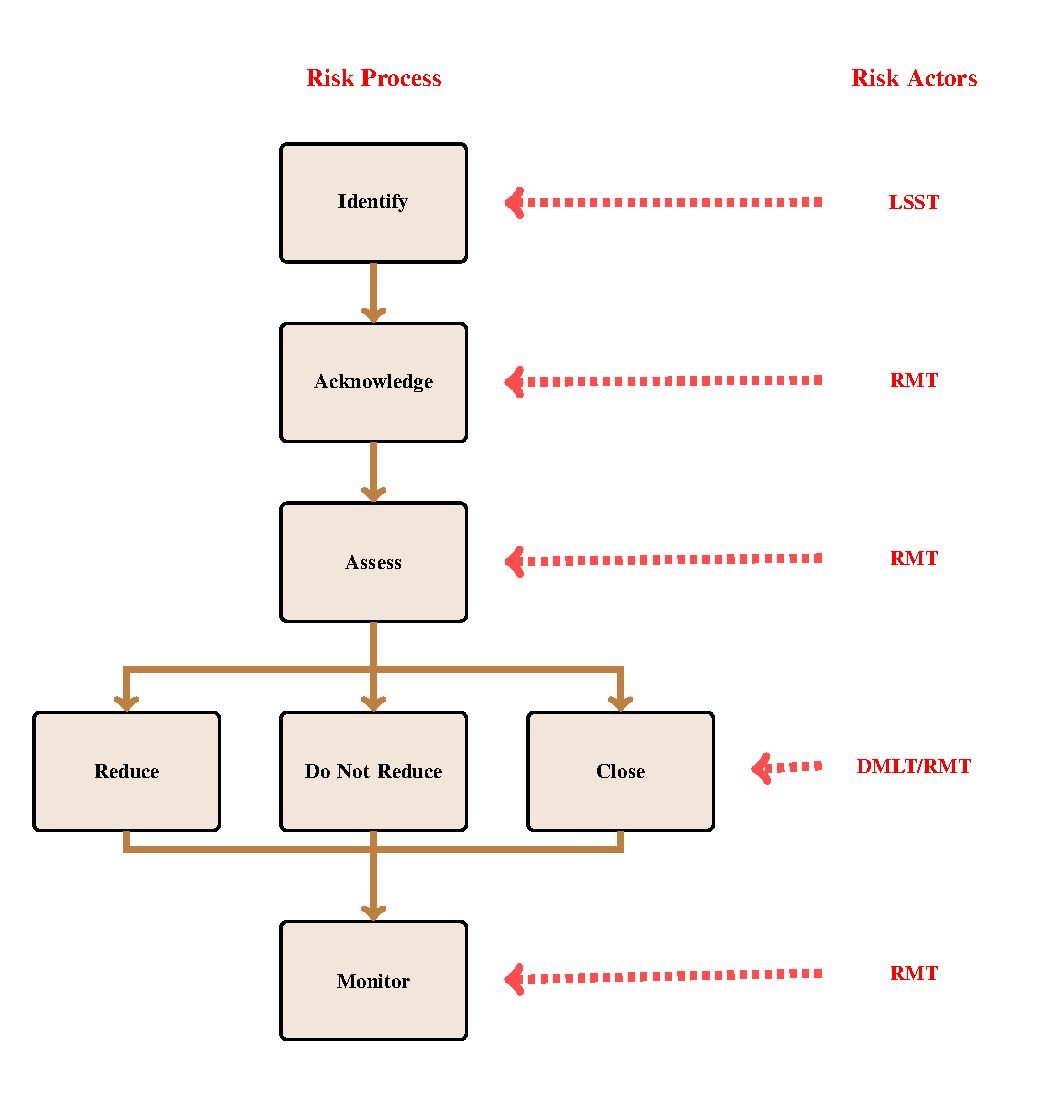
\includegraphics[width=0.8\textwidth]{images/RiskProcess}
\end{center}
\caption{Risk Management Process}
\label{fig:riskprocess}
\end{figure}

\subsubsection*{Task 1: Identify risk scenarios}

It is expected that potential risks will be submitted by various parties in LSST, and indeed input of possible risks should be communicated by the CUs and DPCs.

\subsubsection*{Task 2: Acknowledge the risks}
Any new risks should be reviewed by the risk management team during the risk management meeting to determine their validity. If a new risk is not considered valid, it is closed. The closed risks will be presented to DMLT.
In addition, more general risk scenarios should be contemplated during the risk management meeting to identify any new risks.

\subsubsection*{Task 3: Assess the risks}

For each valid risk, and for all previously identified risks, (re)assess their likelihood and severity, using the scales defined in section \ref{sect:scoring}. The RMT recommends an assessment that the DMLT approves or modifies.

\subsubsection*{Task 4: Reduce the risks}

For those risks that are deemed as "unacceptable", the risk management team will try to define possible actions to reduce risks in terms of occurrence and/or likelihood.
The risk management team needs to balance increasing expenditure to tackle a risk.

All risks ranked as "unacceptable" should have at least one dedicated action.
The RMT should recommend mitigating actions if possible; the DMLT decides on the final actions to be taken, approving the recommendations of the RMT or formulating new actions.

\subsubsection*{Task 5: Do not reduce the risks (acceptance)}

Whether or not mitigation actions are identified, there should come a time in the project when a risk can not be reduced any further. In this case the risk management team should recommend to {\em accept} the risk, even if it does not pass the acceptance criteria defined under task 3.

Risks should also be accepted if the cost to mitigate is greater than the cost of the consequences, obviously. More generally a risk might be accepted if the severity/likelihood of the consequences does not merit the cost to mitigate.

All accepted risks should be re-assessed at the next risk management cycle.

A risk may be closed if it is deemed unnecessary to continue monitoring the risk. This might be because it no longer applies to the project (is no longer a valid risk), or is no longer a significant risk (likelihood is null or no negative consequences). The risk management meeting may identify risks to be recommended for closing.

\subsubsection*{Task 6: Monitor the risks}

After approval, the RMT is in charge of updating and issuing a new version of the Risk register. Feedback from the concerned parties is also necessary so that the risk management team can properly monitor risks. Were recommended actions taken? What were the results? Were risks recommended for acceptance approved or not?

\subsection{Risk management technical implementation \label{sect:technical} }
JIRA has been chosen as our Risk Management Tool in DM, this section describes the technical part of a risk registration and monitoring.

